\documentclass[10pt,a4paper]{article}
\usepackage[utf8]{inputenc}
\usepackage{amsmath}
\usepackage{amsfonts}
\usepackage{amssymb}
\usepackage{makeidx}
\usepackage{graphicx}
\usepackage[obeyspaces]{url}
\author{Rolando Muñoz}
\title{Finder manual}

\begin{document}
\maketitle

\section{Introduction}
Finder is a Praat plug-in for searching annotations in TextGrid files. When a search is completed, you can view and edit the results one-by-one using the Editor window. Alternatively, you can create new files from the matched parts. Use the script template for more specific tasks.
\section{How to install}
To install the plug-in, (1) download the project folder from the Links section and unzip it. Then, (2) find the \textit{Praat Preference} folder. This comes by default when you use Praat for the first time. Depending on you operating system, these could be the locations:

\begin{itemize}
	\item In Linux, go to \path{/home/user name/.praat-dir}
	\item In Mac, go to \path{/Users/user name/Library/Preferences/Praat Prefs/}
	\item In Windows, go to \path{C:\Users\user name\Praat}
\end{itemize}

Now, (3) drop the project folder inside the Preferences folder. Finally, (4) open Praat. In the fixed menu, you should have \path{Praat > Goodies > Finder} as in Figure {\tiny }\ref{fig:finder_menu}\footnote{If Praat was opened at the time you installed the plug-in, you will not see any change. So, close and open it again.}.

\begin{figure}
	\centering
	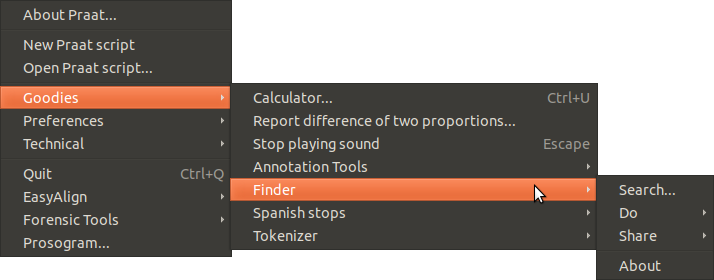
\includegraphics[scale=0.5]{img/004}
	\label{fig:finder_menu}
	\caption{Finder menu}
\end{figure}

\section{Getting started}
The Finder menu is composed of several commands. Use \textbf{Create an index} and \textbf{Search}
\subsection{Create an index}
The first thing to do is creating an index. By doing so, the plug-in will read the information contained
in your TextGrid files and store it internally.
This process will capture the state of your annotations at a given time. So, if later, a TextGrid is modify, it is important to run this command again, in order to include the new changes.

\begin{figure}
	\centering
	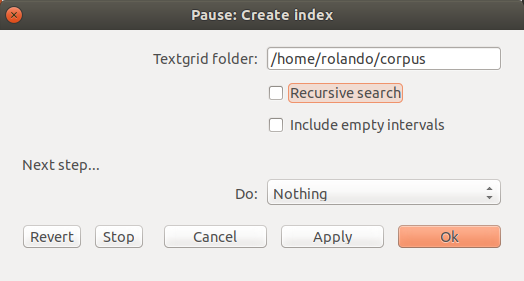
\includegraphics[scale=0.5]{img/001}
	\label{fig:create_index_window}
	\caption{Create index window}
\end{figure}
\subsection{Search}
\subsubsection{Filter}
\subsubsection{Share}
\subsection{Do something}
\subsubsection{View \& Edit files}
\subsubsection{Extract files}
\subsubsection{Open a script template}
\section{Some tips}
\subsection{Create a list of words}

\end{document}